\chapter{Docker}
\label{Docker}
\thispagestyle{empty}

Docker è una piattaforma per sviluppare, spedire e avviare applicazioni usando la tecnologia dei container.

\section{Introduzione}
Il progresso dell'industria tecnologica procede ad un ritmo elevatissimo e sempre più aziende hanno bisogno di strumenti affidabili e facilmente scalabili a seconda delle esigenze. La piattaforma Docker è lo strumento all'avanguardia che permette la consegna ed installazione di servizi in semplicità e sicurezza, mediante componenti leggeri e standard, assai portabili e aggiornabili, chiamati container. Questi non solo sono utilizzati per sviluppare nuovi servizi e micro-servizi, ma anche per eseguire applicazioni esistenti, preparandole ad una futura modernizzazione. Infatti i vantaggi della piattaforma hanno convinto l'industria, che oggi confida sempre più su questa tecnologia, costruendo piattaforme di container.

\section{Versioni}
Docker è un software disponibile per diverse piattaforme fra cui sistemi Linux (Ubuntu, Fedora, Debian, CentOS), Windows, Mac, ma anche in cloud (Amazon Web Services, Microsoft Azure). Sono disponibili due versioni:
\begin{itemize}
    \item Community Edition (CE): gratuita, ideale per sviluppatori singoli e per piccoli team. Possiede le funzionalità di base della piattaforma (engine, orchestration tools, networking e security).
    \item Enterprise Edition (EE): studiata per sviluppo aziendale e per team che sviluppano, spediscono ed eseguono applicazioni essenziali per l'impresa.
\end{itemize}

\section{Architettura e funzionamento}
Docker utilizza funzionalità di virtualizzazione del kernel Linux per avviare servizi e applicazioni in un ambiente isolato, protetto e sicuro. Utilizza \verb|libcontainer| per creare container con namespaces, cgroups, proprietà e filesystem.

In seguito si descriveranno i componenti base di Docker e di come interagiscano fra loro.

\subsection{Immagini}
Un'immagine è un template con istruzioni per la creazione di container. Le immagini descrivono anche i componenti e i programmi all'interno del container e possono includere anche altre immagini. Ad esempio, è possibile indicare che sull'immagine "Ubuntu" sia installato il web server Apache e un'altra applicazione con le relative impostazioni.

È possibile creare le proprie immagini, ma anche utilizzare altre immagini disponibili su Docker Hub. Per creare un immagine è necessario creare un \emph{Dockerfile} che indichi gli step per la creazione e l'avvio dell'immagine. Ogni step costituisce un layer dell'immagine: la ricreazione dell'immagine a fronte di modifiche consisterà nella sola sostituzione dei layer modificati. L'operazione risulta quindi assai conveniente, leggera e veloce.

\subsection{Container}
Un container è un'istanza eseguibile di un'immagine. Ogni container possiede i propri processi, la propria memoria, i propri dispositivi e stack di rete. I container isolano quindi il proprio ambiente da quello esterno, assicurandosi che i propri applicativi funzionino sempre e in modo sicuro, indipendentemente dalle specifiche dell'host. È possibile connettere un container alla rete oppure ad altri container, assegnargli spazio di archiviazione e utilizzare lo stato attuale per creare nuove immagini. Pertanto un container è definito dalla sua immagine, dalla sua configurazione di avvio, ma al riavvio ogni modifica al suo stato o ai dati verrà persa.

Per introdurre la persistenza dei dati è necessario utilizzare \emph{volumi}. Questi sono completamente gestiti da Docker, sono facili da eseguire o migrare e sono utlizzabili in sicurezza da più container. La creazione di un volume consiste nella copia di una directory specifica dal filesystem del container verso il filesystem dell'host. Docker gestisce direttamente il contenuto di queste directory. Ad esempio, a seguito del riavvio di un container Docker carica i dati salvati sull'host all'interno della directory specificata, ripristinando il suo stato prima dello spegnimento.

\subsection{Docker Engine}
Docker Engine è un'applicazione con architettura di tipo client-server. È costituita da tre componenti:
\begin{itemize}
    \item Un processo daemon (\verb|dockerd|) che rappresenta il server.
    \item Una REST API in che modo i programmi possono interagire con il processo daemon.
    \item Un'interfaccia a linea di comando (\verb|docker|) che rappresenta il client.
\end{itemize}
Il daemon riceve richieste API e per gestire container, immagini, reti e volumi e può anche comunicare con altri daemon per gestire servizi Docker più complessi. Il client invece, eseguendo comandi come \verb|docker run|, utilizza le API per comunicare col daemon.

\begin{figure}[ht]
    \centering
    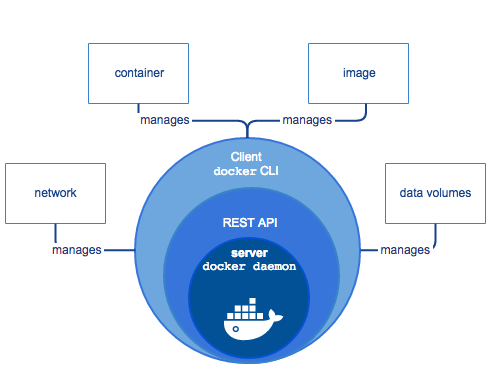
\includegraphics[scale=0.5]{immagini/engine-components-flow.png}
    \caption{Struttura del Docker Engine}
    \label{fig:docker-engine}
\end{figure}

\begin{figure}[ht]
    \centering
    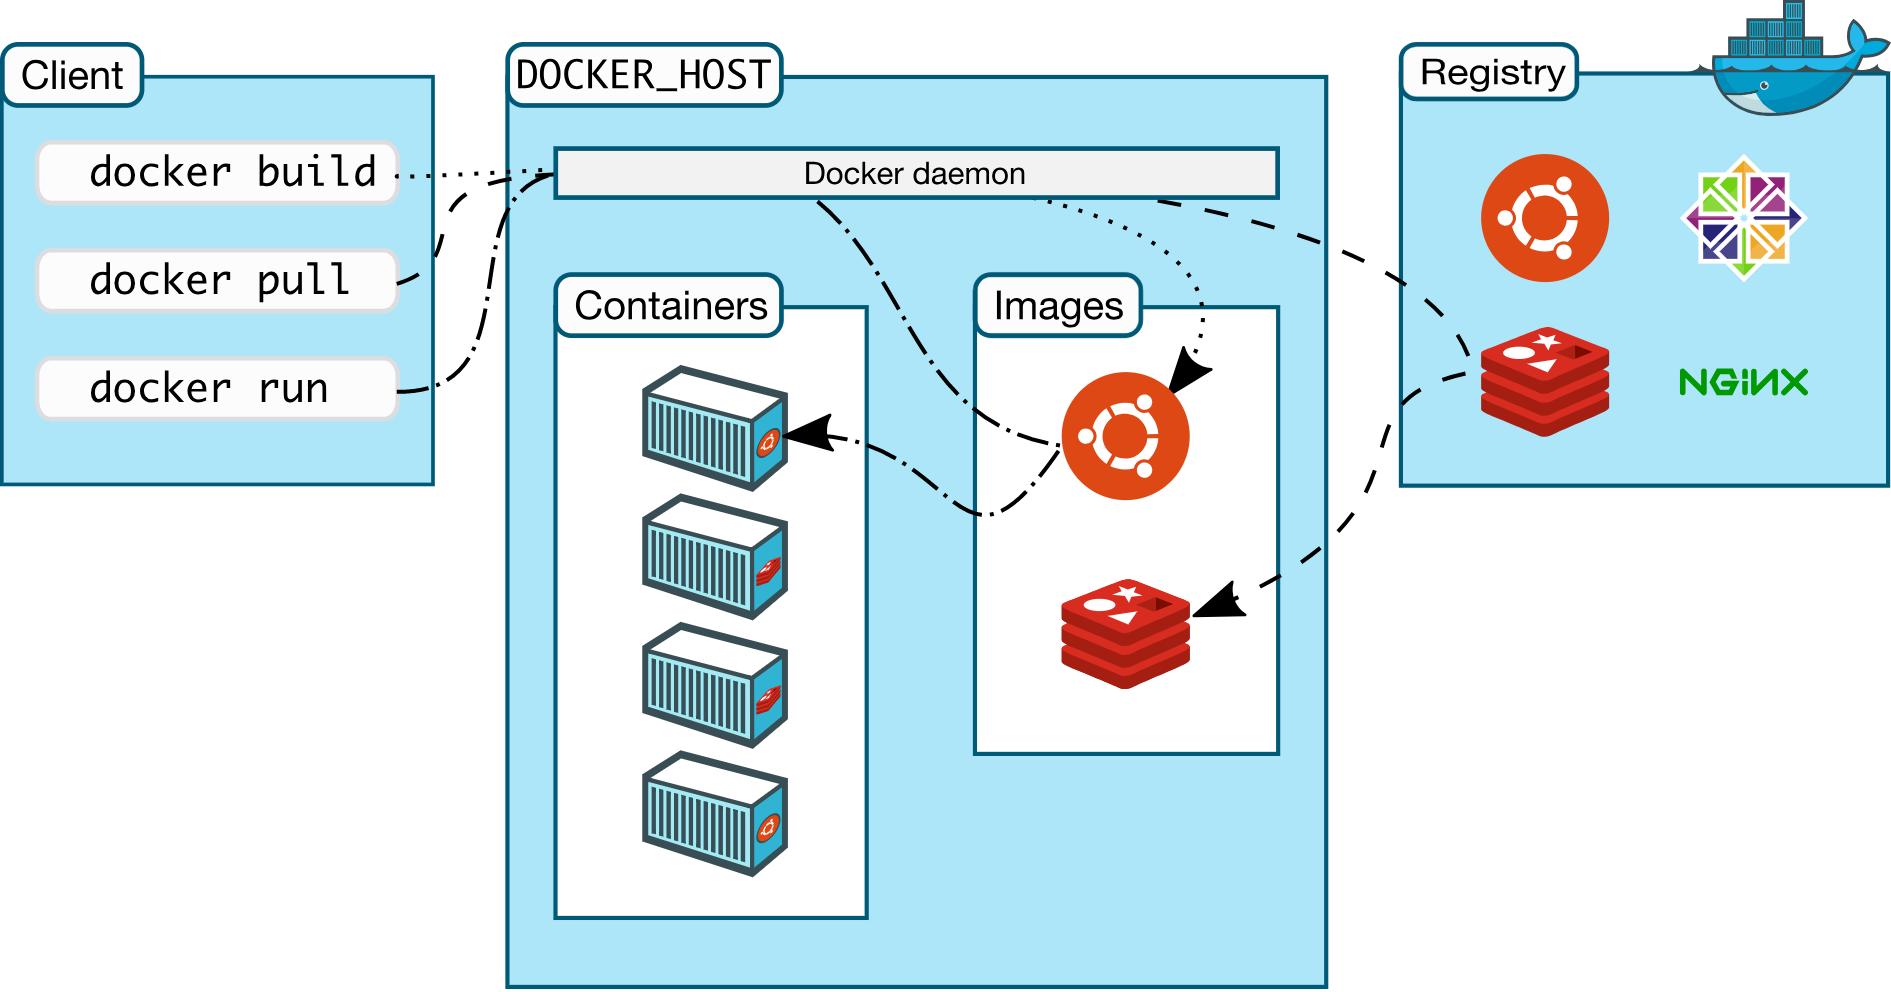
\includegraphics[scale=0.3]{immagini/architecture.png}
    \caption{Esempio funzionamento Docker Engine}
    \label{fig:docker-architecture}
\end{figure}

\subsection{Docker Hub}
Docker Hub è un servizio che consente di collegarsi a repository di container. Permette agli utenti di caricare e scaricare liberamente immagini di container da avviare sui propri host. Costituisce inoltre il nodo centrale per lo sviluppo, la distribuzione e gestione delle modifiche dei container. Docker Hub contiene un gran numero di repository ufficiali, pubblici e certificati dai fornitori. Fra questi si citano Nginx, Redis, MongoDB, Ubuntu, PostgreSQL, Node.js, MySQL, Tomcat e molti altri.

\subsection{Docker Compose}
%%%%% Descrivere docker compose, vantaggi, connettività

%% esempio docker-compose.yml
\lstinputlisting[style=my-bash, lastline=17]{script/docker-compose.yml}

\subsection{}
 
% breve confronto prestazionale fra container e VMs. INCLUDERE QUALCHE IMMAGINE
\section{Vantaggi rispetto alla virtualizzazione}
I container risultano più leggeri rispetto a macchine virtuali perché non necessitano dell'installazione di un sistema operativo guest. Richiedono inoltre meno CPU, RAM e spazio d'archiviazione. Sono infine maggiormente portabili, perché le applicazioni installate funzionano in un ambiente controllato e preparato ad hoc, anziché richiedere hardware e software specifici.
\begin{figure}[ht]
    \centering
    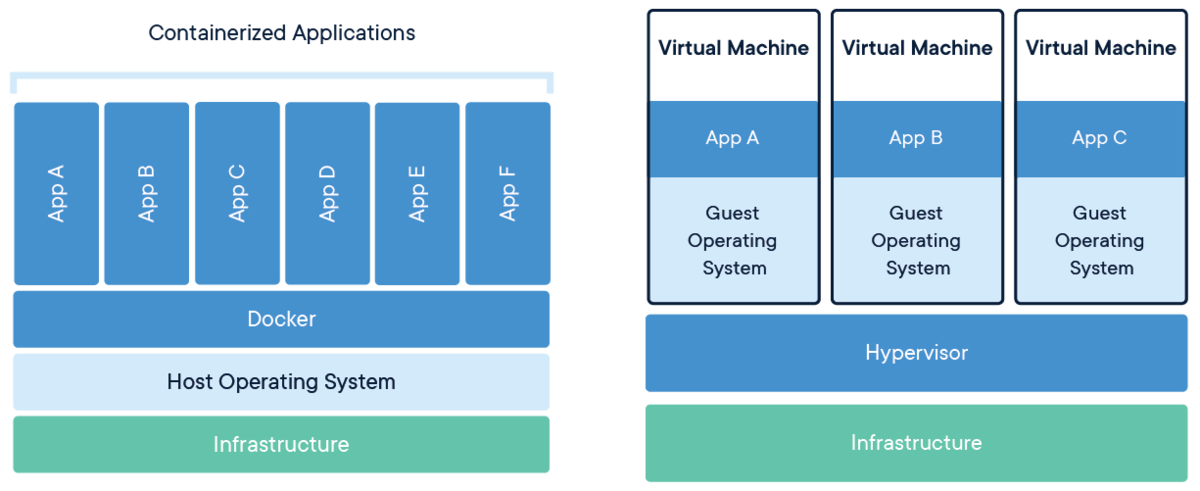
\includegraphics[width=\textwidth]{immagini/docker-containerized-and-vm-transparent-bg.png}
    \caption{Stratificazione di un sistema a container e di un sistema con VMs}
    \label{fig:my_label}
\end{figure}